\section{Resultados}
%Deben incluir los resultados de los experimentos, utilizando el formato m´as adecuado
%para su presentaci´on. Deber´an especificar claramente a qu´e experiencia corresponde
%cada resultado. No se incluir´an aqu´ı corridas de m´aquina.

%     EXPERIMENTACION FUERTEMENTE RELACIONADA AL OPCIONAL
%   --------------------------------------------------------
% \subsection{Experimentación sobre predicados teóricos}
% \subsubsection{El valor de $p$ y el error del sistema}
% Calculamos el error, mediante la aproximación $|Ax' - x'|$, producido con 100 valores distintos de \textit{p}.
% \begin{figure}[H]
%   \centering
%   \includegraphics[ height=10cm, width=12cm]{../experimentacion/cualitativo/completo_distinto_p/p_error}
%   \caption{error de la aproximación sobre el test de 15 segundos}
% \end{figure}


\subsection{Experimentación con estructuras de datos}

Medimos los tiempos al ejecutar 3 veces los tests de la cátedra usando como estructura interna 
un vector y un mapa (\textit{vector} y \textit{map} de la STL de C++).

\begin{figure}[H]
\centering
\includegraphics[ width=12cm, trim=0 3.5cm 0 0,clip]{Imagenes/test_15seg}
\caption{tiempos de \textit{test 15 segundos} con vector y mapa}
\end{figure}

\begin{figure}[H]
\centering
\includegraphics[ width=12cm, trim=0 3.5cm 0 0,clip]{Imagenes/test_30seg}
\caption{tiempos de \textit{test 30 segundos} con vector y mapa}
\end{figure}

Estos tiempos son los indicados por el framework \textit{GTest} al ejecutar los tests en una máquina
de los laboratorios del Departamento.

\subsection{Experimentación cuantitativa}
\subsubsection{Aproximación de la solución}
Computamos la aproximación de la solución x' obtenida con $|Ax' - x'|$ utilizando distintos casos de test:

\begin{table}[H]
\centering
\begin{tabular}{ |c|||c| }
 \hline
 Test & $|Ax' - x'|$ \\
 \hline
 \hline
 trivial & 0 \\
 sin links & 6.2063e-17 \\
 completo & 5.5511e-17 \\
 aleatorio & 7.6163e-07 \\
 aleatorio desordenado & 5.3216e-07 \\
 15 segundos & 5.4199e-07 \\
 30 segundo & 7.9482e-07 \\
 \hline
\end{tabular}
\caption{error de aproximación en tests provistos por la cátedra}
\end{table}

\subsubsection{Error absoluto con respecto a los tests de la cátedra}
Vemos la distancia en norma 2 entre nuestra solución x' y la provista por la cátedra:

\begin{table}[H]
\centering
\begin{tabular}{ |c|||c| }
 \hline
 Test & Error \\
 \hline
 \hline
 trivial & 0 \\
 sin links & 0 \\
 completo & 0 \\
 aleatorio & 0 \\
 aleatorio desordenado & 0 \\
 15 segundos & 5.8256e-07 \\
 30 segundo & 5.8.273e-07 \\
 \hline
\end{tabular}
\caption{distancia entre la solución obtenida y la provista por la cátedra}
\end{table}



\subsection{Experimentación sobre distintas implementaciones}
\subsubsection{Error con distintos tipos de datos para almacenar punto flotante}
Para ver el impacto de usar \textit{float}, \textit{double} o \textit{long double}, calculamos el error al aproximar $|Ax' - x'|$ usando cada uno de estos tipos de datos.

\begin{table}[H]
\centering
\begin{tabular}{ |c||c|c|c| }
 \hline
 Test & float & double & long double \\
 \hline
 \hline
 trivial & 0 & 0 & 0 \\
 sin links & 6.2063e-17 & 6.2063e-17 & 6.2063e-17 \\
 completo & 5.5511e-17 & 5.5511e-17 & 5.5511e-17 \\
 aleatorio & 7.6163e-07 & 7.6163e-07 & 7.6163e-07 \\
 aleatorio desordenado & 5.3216e-07 & 5.3216e-07 & 5.3216e-07 \\
 15 segundos & 5.5818e-07 & 5.4199e-07 & 5.4199e-07 \\
 30 segundo & 8.1439e-07 & 7.9482e-07 & 7.9482e-07 \\
 \hline
\end{tabular}
\caption{error de aproximación con distintos tipos de punto flotante}
\end{table}

Cabe mencionar que en la máquina donde se realizaron estas mediciones, \textit{float} mide 4 bytes, mientras que \textit{double} mide 8 bytes y \textit{long double} mide 16 bytes.

\subsubsection{Error con distintos tipos de sumatoria}
Vemos el impacto de sumar normalmente, sumar ordenando ascendentemente los números, o usar el algoritmo de Kahan, calculando el error al aproximar $|Ax' - x'|$ usando cada uno de estos algoritmos (siempre almacenando los datos en \textit{long double})

\begin{table}[H]
\centering
\begin{tabular}{ |c||c|c|c| }
 \hline
 Test & Normal & Ordenando & Kahan \\
 \hline
 \hline
 trivial & 0 & 0 & 0 \\
 sin links & 6.2063e-17 & 6.2063e-17 & 6.2063e-17 \\
 completo & 5.5511e-17 & 5.5511e-17 & 5.5511e-17 \\
 aleatorio & 7.6163e-07 & 7.6163e-07 & 7.6163e-07 \\
 aleatorio desordenado & 5.3216e-07 & 5.3216e-07 & 5.3216e-07 \\
 15 segundos & 5.4199e-07 & 5.4199e-07 & 5.4199e-07 \\
 30 segundo & 7.9482e-07 & 7.9482e-07 & 7.9482e-07 \\
 \hline
\end{tabular}
\caption{error con distintos algoritmos de sumatoria}
\end{table}

\subsection{Experimentación cualitativa sobre distintas estructuras de grafos}
Para analizar los resultados obtenidos, queremos ver cómo influye la estructura del grafo y el valor de p sobre las distintas estructuras presentadas en la sección Desarrollo.

\subsubsection{Malla}
Calculamos el Page Rank para distintos valores posibles de \textit{p}, dispersos en el intervalo $(0, 1)$:
\begin{figure}[H]
\centering
\includegraphics[ width=12cm, trim=0 3.5cm 0 0,clip]{../experimentacion/cualitativo/malla/malla_distintos_p}
\caption{ranking con distintos valores de \textit{p}}
\end{figure}

\subsubsection{Página popular}
Se calcula el Page rank para $p = 0.65$.

\begin{figure}[H]
\centering
\includegraphics[ height=10cm, width=13cm, trim=0 2cm 0 0,clip]{../experimentacion/cualitativo/pagina_popular/pagina_popular_rank}
\caption{ranking calculado con $p = 0.65$}
\end{figure}

Calculamos el ranking de la páginas más y menos populares del sistema, y su variación en función de $p$.

\begin{figure}[H]
\centering
\includegraphics[ height=10cm, width=12cm]{../experimentacion/cualitativo/pagina_popular/pagina_popular_distintos_p}
\caption{variación de mejor y peor ranking con respecto a p}
\end{figure}

\subsubsection{Escalonado}
Se calcula el Page Rank con $p = 0.65$.

\begin{figure}[H]
\centering
\includegraphics[ height=10cm, width=13cm, trim=0 2cm 0 0,clip]{../experimentacion/cualitativo/escalonado/escalonado_rank}
\caption{ranking calculado con $p = 0.65$}
\end{figure}

Calculamos el ranking de la páginas más y menos populares del sistema, y su variación en función de $p$.

\begin{figure}[H]
\centering
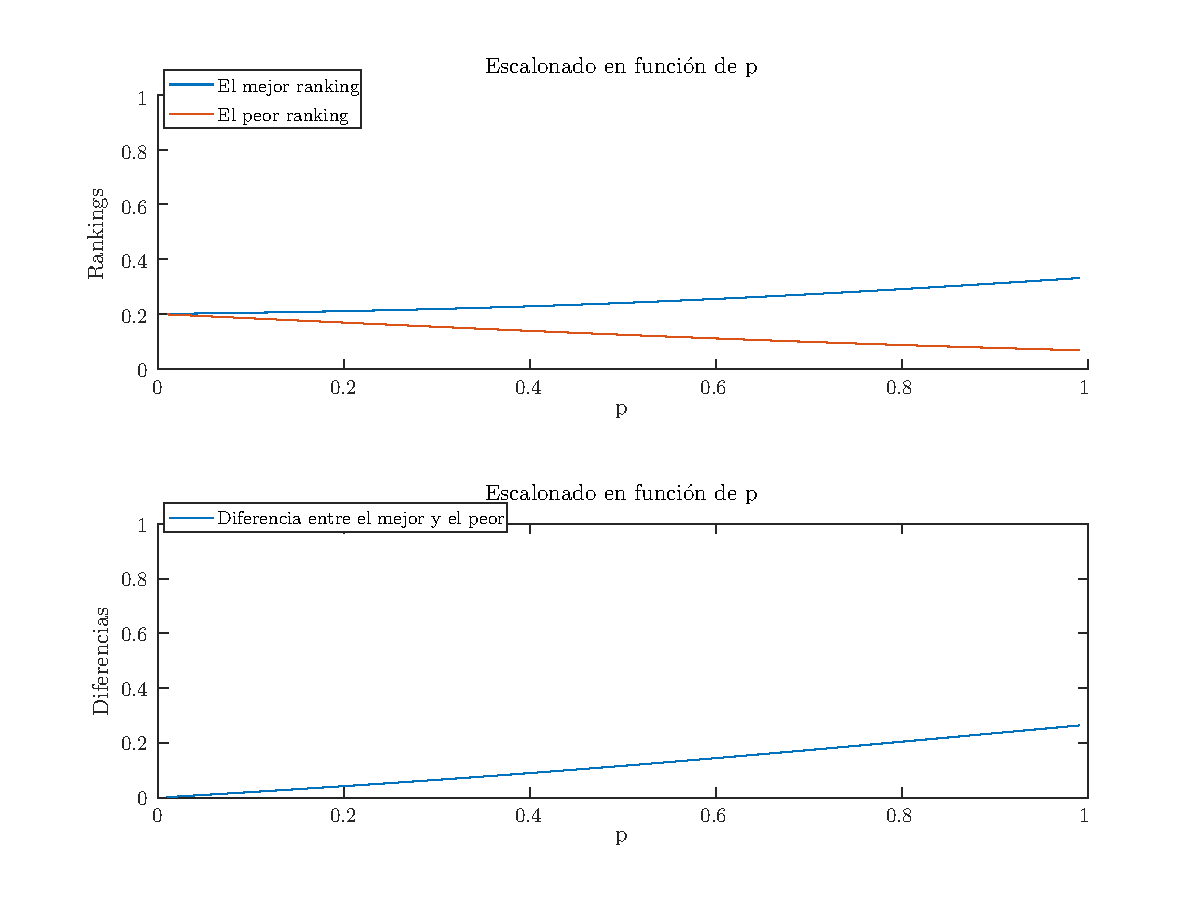
\includegraphics[ height=10cm, width=12cm]{../experimentacion/cualitativo/escalonado/escalonado_distintos_p}
\caption{variación de mejor y peor ranking con respecto a p}
\end{figure}

\subsubsection{Roba éxito}
Se calcula el Page Rank con $p = 0.65$.

\begin{figure}[H]
\centering
\includegraphics[ height=10cm, width=13cm, trim=0 2cm 0 0,clip]{../experimentacion/cualitativo/roba_exito/roba_exito_rank}
\caption{ranking con $p = 0.65$}
\end{figure}
